\clearpage
\phantomsection
\section*{Chương 13. Kiểm chứng ba tầng: float / fixed / RTL}
\addcontentsline{toc}{section}{Chương 13. Kiểm chứng ba tầng: float / fixed / RTL}
\pdfbookmark[1]{Chương 13. Kiểm chứng ba tầng: float / fixed / RTL}{chuong13}

\begin{learningobj}
Sau Chương~13, người học sẽ:
\begin{enumerate}[leftmargin=1.4em]
    \item Vận hành được quy trình kiểm chứng ba tầng: (1)~mô hình float đối chiếu Praat; (2)~mô hình dấu phẩy tĩnh twin đối chiếu float; (3)~RTL/sim đối chiếu twin bit-exact.
    \item Định nghĩa và tính tay được ba chỉ số cổ điển \textbf{GPE}, \textbf{VDE}, \textbf{FFE} (Gross Pitch Error, Voicing Decision Error, Fine/F0 Frame Error) kèm ví dụ số đã kiểm Python.
    \item Viết testbench Avalon-ST có \texttt{valid}-gap và backpressure, đếm beat, so Q12.4 với golden.
    \item Điền bảng tài nguyên từ báo cáo Fitter thật (không bịa số), và giải thích vì sao mỗi tầng bắt một lớp lỗi khác nhau.
\end{enumerate}
\end{learningobj}

\subsection*{13.1. Hiện tượng thật: ba tầng bắt ba lớp lỗi}

\begin{firstprin}{Silicon không chạy Python --- hãy khoanh đúng lớp}
Một đường $F_0$ sai có thể đến từ rất nhiều chỗ: nhầm công thức Boersma, sai Q-format, sai handshake, quên bão hòa, đảo endian. Nếu nhảy thẳng vào Signal Tap trên DE10, bạn sẽ mất ngày để đoán. Ba tầng kiểm chứng tách bạch ba lớp:
\begin{itemize}[leftmargin=1.4em]
    \item \textbf{Tầng 1 --- Float vs Praat:} cùng wav, cùng time step $10\,\text{ms}$, cùng floor/ceiling $75$--$600\,\text{Hz}$. Sai ở đây là sai \emph{thuật toán / thứ tự bước} (quên chuẩn hóa $C[\tau]$, sai parabolic, tắt nhầm silence gate).
    \item \textbf{Tầng 2 --- Fixed twin vs Float:} cùng công thức nhưng mọi phép toán dùng Q$m.n$, round/sat/shift giống RTL. Sai ở đây là sai \emph{lượng tử hóa và làm tròn}.
    \item \textbf{Tầng 3 --- RTL vs Fixed:} ModelSim/Questa hoặc Signal Tap dump từng mẫu/từng khung. Mục tiêu lab: \textbf{$0$ bit mismatch} trên vector golden. Sai ở đây là sai \emph{handshake, latency, reset, X-propagation}.
\end{itemize}
Nhảy thẳng tầng~3 khi tầng~1 còn đỏ chính là lãng phí ngày debug FSM.
\end{firstprin}

Ba vector bắt buộc mọi khối tiền xử lý (đã nêu Chương~3): \texttt{zero} (toàn $0$), \texttt{DC} (hằng khác $0$), \texttt{clip} (đụng $\pm 32767$). Thêm vector sine $75/100/200/440/590\,\text{Hz}$, nhiễu trắng, âm xát $/s/$, và hai đoạn giọng thật --- cùng tinh thần \texttt{verify\_tiers.py}.

\begin{figure}[H]
\centering
\begin{tikzpicture}[font=\small, >=Stealth,
  tier/.style={draw, rounded corners, align=center, minimum width=3.6cm, minimum height=1.15cm}]
  \node[tier, fill=blue!10] (t1) {Tầng 1\\Float $\leftrightarrow$ Praat\\GPE / VDE / FFE};
  \node[tier, fill=teal!10, right=1.1cm of t1] (t2) {Tầng 2\\Fixed $\leftrightarrow$ Float\\sai số cent / Q};
  \node[tier, fill=orange!12, right=1.1cm of t2] (t3) {Tầng 3\\RTL $\leftrightarrow$ Fixed\\bit-exact + beat};
  \draw[->, very thick] (t1)-- (t2);
  \draw[->, very thick] (t2)-- (t3);
  \node[below=0.45cm of t1, font=\scriptsize, align=center]{Công thức\\thứ tự bước};
  \node[below=0.45cm of t2, font=\scriptsize, align=center]{Q-format\\round / sat};
  \node[below=0.45cm of t3, font=\scriptsize, align=center]{Handshake\\latency / X};
\end{tikzpicture}
\caption{Ba tầng kiểm chứng: mỗi tầng khoanh một lớp lỗi; chỉ xuống tầng dưới khi tầng trên đã xanh trên cùng bộ vector.}
\label{fig:ch13_three_tiers}
\end{figure}

\subsection*{13.2. Toán: GPE, VDE, FFE --- định nghĩa từng ký hiệu}

Trong đánh giá cao độ chuẩn (Rabiner, Chu \& Alwan, v.v.), mỗi khung được gắn nhãn hữu thanh/vô thanh bởi tham chiếu (ở đây: Praat) và bởi hệ thống (float / fixed / RTL). Ký hiệu:
\begin{itemize}[leftmargin=1.4em]
    \item $N$: tổng số khung có mặt cả hai hệ thống.
    \item $N_{VV}$: số khung cả tham chiếu lẫn hệ thống đều hữu thanh.
    \item $F_{\mathrm{ref}}[k]$, $F_{\mathrm{hw}}[k]$: cao độ (Hz) trên các khung cùng hữu thanh.
\end{itemize}

\paragraph{GPE --- Gross Pitch Error (Sai cao độ thô).}
\begin{equation}
\label{eq:ch13_gpe}
\mathrm{GPE}=\frac{1}{N_{VV}}\bigl|\bigl\{k\in VV:\ \bigl|F_{\mathrm{hw}}[k]/F_{\mathrm{ref}}[k]-1\bigr|>0{,}2\bigr\}\bigr|.
\end{equation}
Ngưỡng $20\%$ roughly một quãng gần (khoảng lớn hơn sai số tinh). GPE cao thường báo octave error ($F_0/2$ hoặc $2F_0$) --- đúng bệnh Chương~8--10 khi quên $C[\tau]$ hoặc voicing nuốt đỉnh đúng.

\paragraph{VDE --- Voicing Decision Error (Sai quyết định hữu/vô thanh).}
\begin{equation}
\label{eq:ch13_vde}
\mathrm{VDE}=\frac{N_{\mathrm{FV}}+N_{\mathrm{FU}}}{N},
\end{equation}
với $N_{\mathrm{FV}}$ = false voiced (hệ thống báo V khi tham chiếu UV), $N_{\mathrm{FU}}$ = false unvoiced (ngược lại). VDE cao $\Rightarrow$ xem lại ngưỡng $V$, $S$, warmup $P_{\mathrm{global}}$ (Chương~10).

\paragraph{FFE --- F0 Frame Error (gộp).}
Nhiều báo cáo lab định nghĩa FFE là tỷ lệ khung ``hỏng'' theo nghĩa \emph{hoặc} sai voicing \emph{hoặc} GPE trên khung cùng hữu thanh:
\begin{equation}
\label{eq:ch13_ffe}
\mathrm{FFE}=\frac{N_{\mathrm{VDE\ frames}}+N_{\mathrm{GPE\ frames}}}{N}.
\end{equation}
(Một số tài liệu gọi ``Fine Error'' là sai số cent trung bình trên khung \emph{không} GPE; lab này dùng FFE dạng frame-error tổng hợp như trên và ghi rõ trong báo cáo.)

\paragraph{Sai số cent trên khung ``tinh''.}
\begin{equation}
\Delta_{\mathrm{cent}}[k]=1200\log_2\bigl(F_{\mathrm{hw}}[k]/F_{\mathrm{ref}}[k]\bigr).
\end{equation}
Ngân sách lab trên sine/giọng sạch: $\max|\Delta_{\mathrm{cent}}| < 20$---$30$~cent sau khi đã loại khung GPE (nếu có). Mỗi stage (DC, FIR lượng tử, window Q1.15, MAC cắt bit, $C[\tau]$ Q3.13, parabolic, LPM\_DIVIDE, Q12.4) góp vài cent; vượt ngân sách thì lần ngược từ peak về FIR, không đoán.

\subsection*{13.3. Ví dụ tính tay --- chỉ số và cent (đã kiểm Python)}

\paragraph{Cent.} $F_{\mathrm{hw}}=199{,}466\,\text{Hz}$ (parabolic Chương~9), $F_{\mathrm{ref}}=200\,\text{Hz}$:
\[
\Delta_{\mathrm{cent}}=1200\log_2(199{,}466/200)\approx -4{,}629\,\text{cent}.
\]
Nằm trong ngân sách $20$~cent.

\paragraph{Đồ thị nhầm lẫn giả định $N=20$ khung.} Giả sử $N_{VV}=14$, trong đó $2$ khung lệch $>20\%$ (octave); thêm $3$ khung sai voicing (không trùng hai khung GPE):
\[
\mathrm{GPE}=\frac{2}{14}\approx 0{,}1429,\qquad
\mathrm{VDE}=\frac{3}{20}=0{,}15,\qquad
\mathrm{FFE}=\frac{5}{20}=0{,}25.
\]
Script \texttt{verify/verify\_chuong\_10\_14.py} khẳng định các tỷ số này. Trên sine sạch lab, mục tiêu thực tế: $\mathrm{GPE}\approx 0$, $\mathrm{VDE}$ thấp, $|\Delta_{\mathrm{cent}}|<20$.

\paragraph{LSB Q12.4.} Tại $200\,\text{Hz}$, $0{,}0625\,\text{Hz}$ $\approx 0{,}541\,\text{cent}$ --- nhỏ hơn nhiều so với $-4{,}6\,\text{cent}$ của parabolic ở ví dụ trên, nên tầng pack hiếm khi là thủ phạm GPE.


\paragraph{Ví dụ tính tay --- ma trận nhầm lẫn năm khung.}
Cho tham chiếu Praat và hệ thống (Hz; $0$ = UV):
\begin{center}\small
\begin{tabular}{@{}cccccc@{}}\toprule
$k$ & 0 & 1 & 2 & 3 & 4 \\
\midrule
$F_{\mathrm{ref}}$ & $200$ & $200$ & $0$ & $180$ & $0$ \\
$F_{\mathrm{hw}}$ & $199{,}5$ & $100$ & $0$ & $0$ & $50$ \\
Nhãn lỗi & tinh & GPE octave & OK UV & false UV & false V \\
\bottomrule
\end{tabular}
\end{center}
Khung cùng hữu thanh $VV=\{0,1\}$ ($N_{VV}=2$). Khung~$1$ có $|100/200-1|=0{,}5>0{,}2$ $\Rightarrow N_{\mathrm{GPE}}=1$. Sai voicing ở $k=3$ (FU) và $k=4$ (FV) $\Rightarrow N_{\mathrm{VDE}}=2$.
\[
\mathrm{GPE}=\frac{1}{2}=0{,}5,\qquad
\mathrm{VDE}=\frac{2}{5}=0{,}4,\qquad
\mathrm{FFE}=\frac{1+2}{5}=0{,}6.
\]
Script verify khẳng định $N_{\mathrm{GPE}}=1$, $N_{\mathrm{VDE}}=2$ trên đúng vector này.

\begin{figure}[H]
\centering
\begin{tikzpicture}[font=\small]
  \node[draw, fill=green!15, minimum width=2.2cm, minimum height=1.2cm, align=center] at (0,1.3) {TV\\đúng V};
  \node[draw, fill=red!15, minimum width=2.2cm, minimum height=1.2cm, align=center] at (2.6,1.3) {FV\\false V};
  \node[draw, fill=red!15, minimum width=2.2cm, minimum height=1.2cm, align=center] at (0,0) {FU\\false UV};
  \node[draw, fill=green!15, minimum width=2.2cm, minimum height=1.2cm, align=center] at (2.6,0) {TU\\đúng UV};
  \node[rotate=90, left] at (-1.5,0.65) {Tham chiếu};
  \node[above] at (1.3,2.1) {Hệ thống $\to$};
  \node[font=\scriptsize, align=left] at (6.2,0.65)
    {VDE $=(N_{\mathrm{FV}}+N_{\mathrm{FU}})/N$.\\
     GPE chỉ đếm trong ô TV\\khi $|F_{hw}/F_{ref}-1|>0{,}2$.};
\end{tikzpicture}
\caption{Hình 13.4 --- Ma trận hữu/vô thanh: VDE lấy hai ô đỏ; GPE lấy tập con của ô TV.}
\label{fig:ch13_confusion}
\end{figure}

\begin{figure}[H]
\centering
\begin{tikzpicture}[font=\scriptsize, >=Stealth,
  s/.style={draw, rounded corners, align=center, inner sep=3pt}]
  \node[s, fill=blue!10] (wav) {wav};
  \node[s, fill=blue!10, right=8mm of wav] (praat) {Praat\\AC};
  \node[s, fill=teal!10, right=8mm of praat] (flt) {float\\twin};
  \node[s, fill=orange!10, below=10mm of flt] (fix) {fixed\\twin};
  \node[s, fill=red!10, below=10mm of fix] (rtl) {RTL\\sim};
  \draw[->, thick] (wav)--(praat);
  \draw[->, thick] (wav)--(flt);
  \draw[<->, thick] (praat)--node[above]{GPE/VDE} (flt);
  \draw[<->, thick] (flt)--node[right]{cent} (fix);
  \draw[<->, thick] (fix)--node[right]{bit-exact} (rtl);
\end{tikzpicture}
\caption{Hình 13.5 --- Luồng đối sánh tầng 1$\to$2$\to$3 trên cùng wav.}
\label{fig:ch13_flow}
\end{figure}

\begin{figure}[H]
\centering
\begin{tikzpicture}[font=\scriptsize, x=0.7cm, y=0.45cm]
  \foreach \y/\lab in {6/valid, 4.5/ready, 3/data, 1.5/score} {
    \node[left] at (0,\y) {\lab};
  }
  \draw[very thick, blue] (1,5.7)--(1,6.3)--(3,6.3)--(3,5.7)--(4,5.7)--(4,6.3)--(10,6.3);
  \draw[very thick, teal] (1,4.2)--(1,4.8)--(5,4.8)--(5,4.2)--(7,4.2)--(7,4.8)--(10,4.8);
  \node at (2,3) {s0};
  \node at (4.5,3) {s1 giữ};
  \node at (8,3) {s1..};
  \fill[orange] (2,1.5) circle (2pt);
  \fill[orange] (8,1.5) circle (2pt);
  \node[font=\scriptsize, align=center] at (5.5,0.2)
    {TB phải hạ ready ngẫu nhiên; scoreboard chỉ chốt khi beat=1.};
\end{tikzpicture}
\caption{Hình 13.6 --- Testbench Avalon-ST: valid-gap + backpressure; chỉ chấm cam được so golden.}
\label{fig:ch13_tb_wave}
\end{figure}

\begin{figure}[H]
\centering
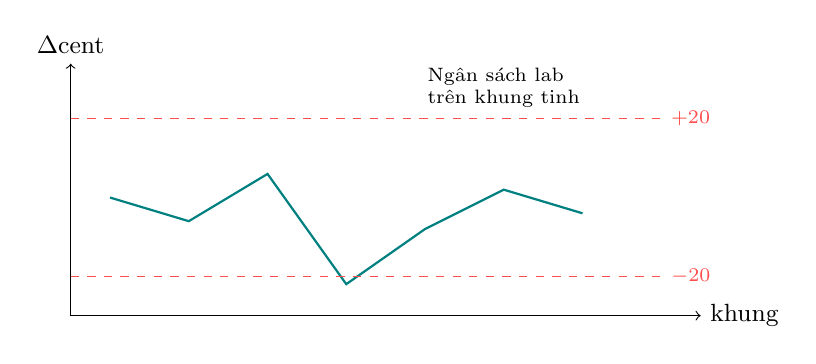
\begin{tikzpicture}[font=\small]
  \draw[->] (0,0)--(8,0) node[right]{khung};
  \draw[->] (0,0)--(0,3.2) node[above]{$\Delta$cent};
  \draw[thick, teal] (0.5,1.5)--(1.5,1.2)--(2.5,1.8)--(3.5,0.4)--(4.5,1.1)--(5.5,1.6)--(6.5,1.3);
  \draw[dashed, red!70] (0,2.5)--(7.5,2.5) node[right,font=\scriptsize]{$+20$};
  \draw[dashed, red!70] (0,0.5)--(7.5,0.5) node[right,font=\scriptsize]{$-20$};
  \node[font=\scriptsize, align=left] at (5.5,2.9){Ngân sách lab\\trên khung tinh};
\end{tikzpicture}
\caption{Hình 13.7 --- Sai số cent khung-tinh phải nằm trong $\pm 20$---$30$~cent sau khi loại GPE.}
\label{fig:ch13_cent_budget}
\end{figure}

\begin{figure}[H]
\centering
\begin{tikzpicture}[font=\scriptsize, >=Stealth,
  b/.style={draw, rounded corners, align=center, minimum width=2.4cm, minimum height=0.85cm}]
  \node[b, fill=red!12] (sym) {Symptom\\GPE cao};
  \node[b, fill=orange!12, right=10mm of sym] (t1) {Tầng 1?\\công thức};
  \node[b, fill=orange!12, right=10mm of t1] (t2) {Tầng 2?\\Q-format};
  \node[b, fill=orange!12, right=10mm of t2] (t3) {Tầng 3?\\handshake};
  \draw[->, thick] (sym)--(t1);
  \draw[->, thick] (t1)--(t2);
  \draw[->, thick] (t2)--(t3);
  \node[below=3mm of t1, align=center]{quên $C[\tau]$\\sai parabolic};
  \node[below=3mm of t2, align=center]{cắt MAC\\ROM endian};
  \node[below=3mm of t3, align=center]{mất beat\\đảo LE};
\end{tikzpicture}
\caption{Hình 13.8 --- Cây chẩn đoán: luôn hỏi tầng trên trước khi đụng Signal Tap.}
\label{fig:ch13_diag_tree}
\end{figure}


\subsection*{13.4. Tầng 1: Float vs Praat}

Thực hành khuyến nghị (Parselmouth hoặc Praat batch):
\begin{verbatim}
snd = parselmouth.Sound(wav, sampling_frequency=16000)
pm = snd.to_pitch_ac(time_step=0.01, pitch_floor=75, pitch_ceiling=600)
f_ref = pm.selected_array["frequency"]  # 0 = UV
# f_float: twin float_pitch_frame tung hop
# Do GPE/VDE/FFE chi tren khung overlap thoi gian
\end{verbatim}
Tham số bắt buộc khớp lab: time step $0{,}01\,\text{s}$, floor $75$, ceiling $600$, và (nếu đối chiếu sâu) cùng voicingThreshold $0{,}45$. Khác tham số $\Rightarrow$ ``sai số'' giả tạo.

\subsection*{13.4b. Tầng 1 sâu: khớp tham số Praat}

Ngoài time step / floor / ceiling, các tham số hay làm lệch giả tạo:
\begin{itemize}[leftmargin=1.4em]
  \item \texttt{voicingThreshold} (mặc định $0{,}45$): khác số $\Rightarrow$ VDE giả.
  \item \texttt{octaveCost} / \texttt{octaveJumpCost}: twin float lab tắt pathFinder thì không so được đường cong ``có Viterbi'' của Praat GUI mặc định --- phải gọi API/\texttt{Pitch.cpp} với cùng cờ tắt, hoặc chấp nhận so trên khung đã voiced ổn định.
  \item Đồng bộ thời gian: tâm cửa sổ lab tại $kH+L/2$; Praat time step $0{,}01\,\text{s}$ phải neo cùng gốc.
\end{itemize}

\paragraph{Ví dụ tính tay --- RTF mô phỏng $1\,\text{s}$.}
Số khung $97$, mỗi khung $\approx 120\,960$ chu kỳ MAC:
\[
T_{\mathrm{proc}}=\frac{120\,960\cdot 97}{50\cdot 10^6}\approx 0{,}2347\,\text{s},
\qquad \mathrm{RTF}\approx 0{,}2347
\]
(RTF = \emph{Real-Time Factor} = thời gian xử lý / thời gian âm thanh; đã kiểm script). Một TB chu kỳ-chính xác cho $1\,\text{s}$ audio vì thế chạy khoảng $0{,}23\,\text{s}$ thời gian mô phỏng xung nhịp (wall-clock phụ thuộc tốc độ sim).

\subsection*{13.5. Tầng 2: Fixed twin vs Float}

Twin cố định bit dùng cùng ROM Hanning Q1.15, ROM $C[\tau]$ Q3.13, cùng sat/shift như RTL. Đo:
\begin{itemize}[leftmargin=1.4em]
    \item Sai lệch cent trung bình / max giữa $F_{\mathrm{fixed}}$ và $F_{\mathrm{float}}$ trên khung cùng voiced;
    \item Số khung đổi voicing so với float (thường $0$ trên sine).
\end{itemize}
Nếu tầng~1 xanh mà tầng~2 đỏ: nghi ngờ cắt bit MAC, quên dịch BFP (\emph{Block Floating Point} --- mỗi khối FFT chia sẻ một exponent; nếu dùng FFT IP), hoặc ROM $C[\tau]$ sai endian trong hex.

\subsection*{13.5b. Tầng 2 sâu: nguồn cent cố định bit}

Mỗi khối góp sai số lượng tử xấp xỉ (thứ tự độ lớn, không phải định lý):
\begin{itemize}[leftmargin=1.4em]
  \item Window Q1.15: hệ số mép khung lệch $1$ LSB $\to$ vài cent.
  \item MAC cắt về thanh ghi trung gian: nếu cắt quá sớm trước khi nhân $C[\tau]$, đỉnh $\tau$ lớn bị thiên vị.
  \item ROM $C[\tau]$ Q3.13: sai endian hex $\to$ GPE hàng loạt (lớp này đôi khi lộ sớm ở tầng~1 nếu float cũng đọc nhầm hex --- tách test ROM).
  \item LPM\_DIVIDE làm tròn quotient: thường $<1\,\text{cent}$ tại $200\,\text{Hz}$.
  \item Pack Q12.4: LSB $\approx 0{,}54\,\text{cent}$ tại $200\,\text{Hz}$.
\end{itemize}
Tổng ngân sách $20$--$30\,\text{cent}$ là ``hộp'' chứa cho cả chuỗi; vượt hộp thì lần từ pack ngược về FIR, đo cent từng điểm neo (sau window, sau MAC, sau $C[\tau]$, sau DIV).

\subsection*{13.6. Tầng 3: RTL vs Fixed --- bit-exact và testbench}

\paragraph{Hợp đồng bit-exact.} Trên cùng \texttt{golden\_pcm.hex}, mọi khung Q12.4 dump từ sim phải bằng twin fixed: $0$ bit lệch. Không ``gần đúng'' ở tầng này.

\paragraph{Testbench Avalon-ST.}
\begin{itemize}[leftmargin=1.4em]
    \item Đọc PCM hex $\to$ stream sample với \texttt{valid} có gap ngẫu nhiên (LFSR).
    \item Sink hạ \texttt{ready} ngẫu nhiên ở mọi stage (đặc biệt MAC$\leftrightarrow$peak, pack$\leftrightarrow$HPS).
    \item Đếm beat vào $=$ đếm beat ra (trừ decimate cố ý).
    \item Scoreboard so $F_q$ với \texttt{golden\_f0.hex}.
    \item Vector cạnh: zero / DC / clip phải cho $F_q=0$ hoặc hành vi DC-blocker đã định nghĩa (Chương~3).
\end{itemize}

\begin{verbatim}
delta_cent = 1200 * np.log2(f_hw / f_praat)
assert np.nanmax(np.abs(delta_cent[voiced_both])) < 20.0
assert (q_rtl == q_fixed).all()  # tang 3
\end{verbatim}

\paragraph{Tài liệu Intel cần mở đúng số.} Avalon~683091, FIR~683208, FFT~683374 (nếu bật), LPM\_DIVIDE handbook. Fmax/ALM/DSP/M10K lấy từ \emph{Fitter report} sau Place \& Route --- không bịa.

\subsection*{13.6b. Tầng 3 sâu: X-propagation và reset}

RTL sim phải:
\begin{enumerate}[leftmargin=1.4em]
  \item Khởi động \texttt{rst\_n}$=0$ đủ vài chu kỳ; mọi thanh ghi median/FSM về $0$.
  \item Không để \texttt{X} (trạng thái chưa xác định trong mô phỏng RTL --- bit chưa được gán $0/1$ sau reset) trên \texttt{valid}/\texttt{ready}: một \texttt{X} làm scoreboard ``xanh giả'' hoặc đỏ ngẫu nhiên.
  \item Dump $F_q$ chỉ khi beat OUT; so với \texttt{golden\_f0.hex} từ twin fixed cùng seed LFSR cho ready.
  \item Vector cạnh zero/DC/clip: kỳ vọng $F_q=0$ (hoặc hành vi DC-blocker đã khóa Chương~3).
\end{enumerate}

\subsection*{13.6c. Golden hex và tái lập bit-exact}

Mỗi revision RTL phải kèm:
\begin{itemize}[leftmargin=1.4em]
  \item \texttt{golden\_pcm.hex} --- vector vào (hoặc WAV gốc + script gen).
  \item \texttt{golden\_f0.hex} --- chuỗi $F_q$ từ twin fixed cùng tham số.
  \item Seed LFSR cho valid-gap/ready trong TB (ghi vào header test).
\end{itemize}
Không tái lập được seed thì ``bit-exact hôm qua'' không chứng minh được hôm nay. Khi đổi $V$, $S$, hoặc ROM $C[\tau]$, phải regenerate golden và ghi chú DIFF.

\paragraph{Ví dụ tính tay --- ngưỡng GPE $20\%$.}
Tại $F_{\mathrm{ref}}=200\,\text{Hz}$, biên GPE là $160$ và $240\,\text{Hz}$. Mọi ước lượng trong $(160,240)$ trên khung VV \emph{không} tính GPE (chỉ đóng góp cent tinh). Octave đúng $100$ hoặc $400$ nằm ngoài biên --- GPE chắc chắn. Đó là lý do GPE cao thường chỉ thẳng ROM $C[\tau]$ hoặc voicing nuốt đỉnh đúng rồi bám hài.

\paragraph{FFE và báo cáo.} Khi viết báo cáo lab, luôn định nghĩa FFE một lần (công thức~\eqref{eq:ch13_ffe}) và không trộn với ``fine error trung bình cent''. Người chấm cần biết bạn đang đếm \emph{tỷ lệ khung hỏng} chứ không phải trung bình cent.

\begin{physicalinsight}
Ba tầng không phải nghi thức nộp bài. Chúng là cách khoanh vùng nhanh: công thức, lượng tử, hay dây nối. Một TB ``end-to-end đỏ'' không nói bạn sửa chỗ nào; ba đèn xanh/đỏ nói được.
\end{physicalinsight}

\subsection*{13.7. Bảng tài nguyên (điền từ Fitter)}

\begin{center}\small
\begin{tabular}{@{}lcccc@{}}\toprule
Khối & ALM & DSP & M10K & Latency (ck) \\
\midrule
PLL + I\textsuperscript{2}S &  &  &  & \\
DC-blocker &  &  &  & \\
FIR $2/3$ &  &  &  & \\
Sliding RAM &  &  &  & \\
Window &  &  &  & \\
MAC ACF &  &  &  & \\
ROM $C[\tau]$ &  &  &  & \\
Peak + DIV &  &  &  & \\
Voicing + median-3 &  &  &  & \\
FSM + pack Q12.4 &  &  &  & \\
\midrule
\textbf{Tổng} (mục tiêu $\lesssim 850$ ALM, $3$ DSP, $4$ M10K) &  &  &  & \\
\bottomrule
\end{tabular}
\end{center}

\noindent Khi nộp bài (Chương~14), không được để trống các ô tổng nếu đã chạy Fitter --- điền số thật kèm ảnh chụp report.

\begin{costbox}
\textbf{Ngân sách xác minh --- giải thích từng mục.}
\begin{itemize}[leftmargin=1.2em]
    \item \textbf{Thời gian sim:} vài giây đến vài phút cho $1\,\text{s}$ audio @ $50\,\text{MHz}$ TB (tuỳ độ chi tiết dump).
    \item \textbf{Disk:} golden hex vài MB --- commit cùng revision RTL để tái lập.
    \item \textbf{Người:} không bỏ tầng float; mỗi fail gắn đúng tầng (GPE $\to$ thuật toán; cent fixed $\to$ Q-format; bit mismatch $\to$ RTL).
    \item \textbf{Vì sao ba tầng:} một TB ``tất cả'' không chỉ ra \emph{loại} lỗi; tách tầng rút ngắn chu kỳ sửa.
\end{itemize}
\end{costbox}


\subsection*{13.7b. Cách điền Fitter thật}

Sau Place \& Route trên Quartus Standard/Lite cho part \texttt{5CSXFC6D6F31C6N}:
\begin{enumerate}[leftmargin=1.4em]
  \item Mở \emph{Fitter $\to$ Resource Usage Summary}: copy ALM logic, DSP blocks, M10K.
  \item Mở \emph{Timing Analyzer}: Fmax của clock $50\,\text{MHz}$ (hoặc clock datapath thật).
  \item Breakdown theo hierarchy nếu tool cho phép --- tách MAC, FIR, FSM.
  \item Không lấy số từ Synthesis sớm (trước Fitter) làm số nộp: synthesis ước tính, Fitter mới là silicon mapping.
\end{enumerate}
Mục tiêu Chương~0: $\lesssim 850$ ALM, $3$ DSP, $4$ M10K, RTF $\approx 0{,}24$. Vượt M10K thường do FIFO/RAM thừa; vượt DSP do nhân cửa sổ + MAC + FIR không chia sẻ --- xét time-multiplex trước khi xin thêm.


\subsection*{13.7c. Liên hệ RTF, sim wall-time và Signal Tap}

RTF $\approx 0{,}23$ trên $1\,\text{s}$ audio nghĩa là mô phỏng chu kỳ-chính xác ``bắt kịp'' nhanh hơn realtime trên giấy; nhưng ModelSim/Questa có thể chậm hơn realtime tường vì diễn dịch. Đừng nhầm wall-time sim với RTF silicon. Signal Tap trên board đo realtime thật: nếu FIFO đầy liên tục, backpressure đang ăn biên $377\,000$ chu kỳ --- cần giảm dump hoặc tăng FIFO, không thêm DSP.

\paragraph{Ví dụ tính tay --- đếm khung overlap thời gian.} Praat và twin phải so trên cùng tập thời điểm. Nếu Praat trả $100$ khung và twin $97$ khung cho $1\,\text{s}$ (do neo cửa khác), chỉ lấy giao khoảng thời gian chung, ví dụ $90$ khung giữa. Tính GPE/VDE trên $N=90$ đó; không pad $0$ giả vào đuôi. Sai bước này tạo VDE giả ở biên câu.

\paragraph{Chuẩn bị báo cáo.} Mỗi tầng một mục: lệnh chạy, tham số, bảng chỉ số, kết luận xanh/đỏ. Đính kèm hash git của RTL + twin + golden. Người chấm tái lập được thì điểm phương pháp mới vững.

\paragraph{Trước khi sang Chương~14.} Tầng~1 cần GPE$\approx 0$ trên sine sạch; tầng~2 max cent $<20$; tầng~3 không lệch bit và đếm beat khớp. Ngoài zero/DC/clip/sine, giữ một đoạn xát vô thanh (ví dụ $/s/$) và một đoạn giọng có thanh điệu --- tránh VDE ``xanh giả'' vì toàn hữu thanh, và để Pearson có nghĩa.


\subsection*{13.8. Bài tập và lời giải giải thích}

\paragraph{Bài tập 13.1.} Chạy twin DC-blocker trên zero / DC / clip. Kỳ vọng đầu ra định tính?

\paragraph{Lời giải.} Zero $\to$ zero. DC hằng $\to$ sau vài hằng số thời gian $\alpha$, đầu ra $\to 0$ (zero tại $z=1$). Clip $\pm 32767$ xen kẽ $\to$ không được wrap thành âm lớn; sat\_16 giữ biên. Nếu clip tạo dao động limit-cycle, nghi \texttt{y\_acc} quá hẹp (Chương~3).

\paragraph{Bài tập 13.2.} Cố ý đảo endian Q12.4 trên golden $200\,\text{Hz}$. GPE/cent thay đổi thế nào?

\paragraph{Lời giải.} Server đọc $2048{,}75\,\text{Hz}$ (Chương~12). $|2048{,}75/200-1|\gg 0{,}2$ $\Rightarrow$ mọi khung đó thành GPE; $\Delta_{\mathrm{cent}}$ khổng lồ. Tầng~1 ``đỏ'' dù thuật toán đúng --- phải bắt bằng test pack/unpack trước khi đổ tội MAC.

\paragraph{Bài tập 13.3.} Cho $N=20$, $N_{VV}=14$, $2$ GPE, $3$ VDE (rời nhau). Tính GPE, VDE, FFE.

\paragraph{Lời giải.} $\mathrm{GPE}=2/14\approx 0{,}1429$, $\mathrm{VDE}=3/20=0{,}15$, $\mathrm{FFE}=5/20=0{,}25$ --- khớp script verify.
